\documentclass[12pt,letterpaper]{report}
\usepackage{natbib}
\usepackage{geometry}
%\usepackage{fancyheadings} fancyheadings is obsolete: replaced by fancyhdr. JL
\usepackage{fancyhdr}
\usepackage{afterpage}
\usepackage{graphicx}
\usepackage{amsmath,amssymb,amsbsy}
\usepackage{dcolumn,array}
\usepackage{tocloft}
\usepackage{template_code/asudis}
\usepackage{fancyvrb} % verbatim replacement that allows latex
\usepackage{verbatim} % verbatim replacement that allows latex

    %%
    % begin Used by ipython notebooks converted
    %%

r


\usepackage[breakable]{tcolorbox}
\usepackage{parskip} % Stop auto-indenting (to mimic markdown behaviour)

\usepackage{iftex}


% Basic figure setup, for now with no caption control since it's done
% automatically by Pandoc (which extracts ![](path) syntax from Markdown).
\usepackage{graphicx}
% Maintain compatibility with old templates. Remove in nbconvert 6.0
% Ensure that by default, figures have no caption (until we provide a
% proper Figure object with a Caption API and a way to capture that
% in the conversion process - todo).
\usepackage{caption}
\DeclareCaptionFormat{nocaption}{}
\captionsetup{format=nocaption,aboveskip=0pt,belowskip=0pt}

\usepackage[Export]{adjustbox} % Used to constrain images to a maximum size
\adjustboxset{max size={0.9\linewidth}{0.9\paperheight}}
\usepackage{float}
\floatplacement{figure}{H} % forces figures to be placed at the correct location
\usepackage{xcolor} % Allow colors to be defined
\usepackage{enumerate} % Needed for markdown enumerations to work
\usepackage{geometry} % Used to adjust the document margins
\usepackage{amsmath} % Equations
\usepackage{amssymb} % Equations
\usepackage{textcomp} % defines textquotesingle
% Hack from http://tex.stackexchange.com/a/47451/13684:

\usepackage{upquote} % Upright quotes for verbatim code
\usepackage{eurosym} % defines \euro
\usepackage[mathletters]{ucs} % Extended unicode (utf-8) support
\usepackage{fancyvrb} % verbatim replacement that allows latex
\usepackage{grffile} % extends the file name processing of package graphics 
% to support a larger range


% The hyperref package gives us a pdf with properly built
% internal navigation ('pdf bookmarks' for the table of contents,
% internal cross-reference links, web links for URLs, etc.)
\usepackage{hyperref}
% The default LaTeX title has an obnoxious amount of whitespace. By default,
% titling removes some of it. It also provides customization options.
\usepackage{titling}
\usepackage{longtable} % longtable support required by pandoc >1.10
\usepackage{booktabs}  % table support for pandoc > 1.12.2
\usepackage[inline]{enumitem} % IRkernel/repr support (it uses the enumerate* environment)
\usepackage[normalem]{ulem} % ulem is needed to support strikethroughs (\sout)
% normalem makes italics be italics, not underlines
\usepackage{mathrsfs}

%%
% End Used by ipython notebooks converted
%%
    

\begin{document}
%-----------------------front matter
\pagenumbering{roman}
\title{Data Driven Neural Model Optimization}
\author{Russell Jarvis}
\degreeName{Doctor of Philosophy}
\paperType{Dissertation}
\defensemonth{Some month}
\gradmonth{Some other month}
\gradyear{Some year}
\chair{Your chair}
\memberOne{Your first member}
\memberTwo{Your second member}
\memberThree{Your third member}
\memberFour{Your fourth member}

\maketitle
\doublespace
%\chapter*{ABSTRACT}
%\chapterstyle{ASU}
%\pagestyle{ASU}
%\frontmatter

%\begin{center}
%    ABSTRACT
%\end{center}
%\begin{abstract}
%\setlength{\parindent}{.5in} 
%\indent 
\hspace*{\parindent} 
Neuron models that behave like their biological counterparts are essential for computational neuroscience.
Reduced neuron models, which abstract away biological mechanisms in the interest of speed and interpretability, have received much attention due to their utility in large scale simulations of the brain, but little care has been taken to ensure that these models exhibit behaviors that closely resemble real neurons.
In order to improve the verisimilitude of these reduced neuron models, I developed an optimizer that uses genetic algorithms to align model behaviors with those observed in experiments.
I verified that this optimizer was able to recover model parameters given only observed physiological data; however, I also found that reduced models nonetheless had limited ability to reproduce all observed behaviors, and that this varied by cell type and desired behavior.
These challenges can partly be surmounted by carefully designing the set of physiological features that guide the optimization. In summary, we found evidence that reduced neuron model optimization had the potential to produce reduced neuron models for only a limited range of neuron types.
%\end{abstract}

%Abstract
%Type ABSTRACT in all capital letters; not bolded, center aligned

%One double-spaced between “ABSTRACT” and text

%Double space all text following; no bold; no italics or underline (used only for species, genre, book titles, musical compositions or foreign words and phrases)

%All acronyms or abbreviations must be written out fully at first use with acronym/abbreviation in parenthesis

%Same size and font as text

%Must start on page i

% Do not exceed 350 words in length


%% Jimmy flagged this sentence.

%%

%\setcounter{page}{i}

\pagenumbering{roman}






%For the three types of reduced neuronal model we were able to obtain models that produced mostly biologically plausible measurements, however, approximately one in every eight fitness constraints needed to be pushed towards the outer limit of plausibility, in-order to produce "all-round" empirically valid cell models. Existing model fitting approaches have succeeded in fitting reduced neuronal models to the onset frequency and exact times of neuron firing, in this work we sometimes fitted to spike timing, but we prioritized other electrical measurements in cells relating to membrane impedance, action potential shape, and current vs firing frequency relationships.\\
%In order to investigate how well reduced models can reproduce experimental data we executed numerical simulations, and coupled the simulations with a genetic algorithm workflow. We used data sourced from neuroelectro.org, and 
%Among alternative models such as Point-process spike chain surrogates, and  multi compartment conductance models, only reduced neuronal models are faster to execute, and easier to interpret. 

%Three subtypes of reduced neuronal models, represent a midway point, in terms of their ability to faithfully reproduce experimental findings.\\
%combined it with a selection of differential equation solvers. custom written differential equation solvers for the Adaptive Exponential, Izhikevich, and simple conductance based models.\\
% Reduced models are a crucial component of many large scale brain simulations.
%in these fast to execute models. 
%We wanted to understand the limits of fitting reduced neural models to experimental electrophysiology measurements, and to use this knowledge to acquire the best possible fits between reduced neuron models and experimental electrical measurements.


%. in this class of models. \\
%\\

%We computed normalized Z-scores.

% * The methods were using a genetic algorithms to solve multiobjective optimization problem. Forward euler solvers


% Additionally reduced neuronal models simulate current flow, and thus are compatible with local field potential models. Although they are not spatially 


% Fulfil and understand the limits of reduced model fitting and agreeing to experiments. 

%as best as possible, fit reduced neural models to experimental measurements, and then to understand and describe limitations in models, that stop impede fitting and cause disagreement between models and experimental measurements.
%of the agreement between reduced neural models and experimental data reproduce experimentally observed neural measurements.
%Since This also involved exploring limitations in some types of neural data.
%* Euclidiating the limits of reduced models and the limits of data, that impede model fitting.
%* Euclidiating model measurement challenges (Rheobase as a soft constraint, threshold computations).
%to data. I
%METHODS 

% It is not novel to embed numerical model simulation inside genetic algorithms, but it is novel recompute rheobase at every sampled model parameter set, and thus to promote a diverse array of model types to the possibility of single spike waveform shape checking.


%Your research problem and objectives
%    Your methods
%    Your key results or arguments: python, numba, dask, dashboard, multiobjective optimisation, open source, reproducibility.
%    Your conclusion
\dedicationpage{}
\include{chapters/ack}
\tableofcontents
% This puts the word "Page" right justified above everything else.
\addtocontents{toc}{~\hfill Page\par}
% Asking LaTeX for a new page here guarantees that the LOF is on a separate page
% after the TOC ends.
\newpage
% Making the LOT and LOF "parts" rather than chapters gets them indented at
% level -1 according to the chart: top of page 4 of the document at
% ftp://tug.ctan.org/pub/tex-archive/macros/latex/contrib/tocloft/tocloft.pdf
\addcontentsline{toc}{part}{LIST OF TABLES}
\renewcommand{\cftlabel}{Table}
\listoftables
% This gets the headers for the LOT right on the first page.  Subsequent pages
% are handled by the fancyhdr code in the asudis.sty file.
\addtocontents{lot}{Table~\hfill Page \par}
\newpage
\addcontentsline{toc}{part}{LIST OF FIGURES}
\addtocontents{toc}{CHAPTER \par}
\renewcommand{\cftlabel}{Figure}
\listoffigures
% This gets the headers for the LOF right on the first page.  Subsequent pages
% are handled by the fancyhdr code in the asudis.sty file.
\addtocontents{lof}{Figure~\hfill Page \par}
%-----------------------body
\doublespace
\pagenumbering{arabic}


Multiple constraining factors effect the design of large scale cortical brain simulations, these are: simulation time, empirical validity, understand-ability and reproducibility. A class of digital neuronal models: "Reduced Neural models", are faster and easier to interpret than multicompartment conductance based models. Reduced models are one of multiple model types used in brain simulations, and they are often utilized as a buffer, for parts of simulations when poorer standards of model/experiment agreement seem tolerable. Large scale cortical brain simulations could be improved if higher standards of model/experiment agreement were satisfied in reduced neuronal models as well as in multi-compartment neurons, as this could bring about more accurate simulations for the same rapid simulation speed. Motivated by the promise of good speed and improved accuracy we used numerical simulations on reduced models inside a genetic algorithm data fitting framework. To explore the upper limit of model/experimental agreement, and thereby obtain experimental fits at the highest possible quality. Unsurprisingly Reduced neuronal models were not unlimited in their flexibility and fidelity. For the three types of reduced neuronal model we were able to obtain models that produced mostly biologically plausible measurements, for six or seven out of eight fitness criteria. Almost consistently one or two in every eight measurement needed to be compromised; pushed outside of the range of plausability, in-order to produce an "all-round" empirically valid cell model. In contrast with existing approaches that have succeeded in fitting reduced neuronal models to the onset frequency and exact times of neuron firing, in this work we disregarded spike timing, and instead fitted models to voltage shapes of recorded from appropriate neuronal membranes\\
\\ 
Among alternative models such as Point-process spike chain surrogates, and  multi compartment conductance models, reduced neuronal models are most often the faster to execute, and easier to interprete. Three subtypes of reduced neuronal models, represent a midway point, in terms of their ability to faithfully reproduce experimental findings.\\
\\
In order to investigate how well reduced models can reproduce experimental data we executed numerical simulations, and coupled the simulations with a genetic algorithm workflow. We used data sourced from neuroelectro.org, and 

%combined it with a selection of differential equation solvers. custom written differential equation solvers for the Adaptive Exponential, Izhikevich, and simple conductance based models.\\
\\


% Reduced models are a crucial component of many large scale brain simulations.

%in these fast to execute models. 
%We wanted to understand the limits of fitting reduced neural models to experimental electrophysiology measurements, and to use this knowledge to acquire the best possible fits between reduced neuron models and experimental electrical measurements.


%. in this class of models. \\
%\\

%We computed normalized Z-scores.

% * The methods were using a genetic algorithms to solve multiobjective optimization problem. Forward euler solvers


% Additionally reduced neuronal models simulate current flow, and thus are compatible with local field potential models. Although they are not spatially 


% Fulfil and understand the limits of reduced model fitting and agreeing to experiments. 

%as best as possible, fit reduced neural models to experimental measurements, and then to understand and describe limitations in models, that stop impede fitting and cause disagreement between models and experimental measurements.
%of the agreement between reduced neural models and experimental data reproduce experimentally observed neural measurements.
%Since This also involved exploring limitations in some types of neural data.
%* Euclidiating the limits of reduced models and the limits of data, that impede model fitting.
%* Euclidiating model measurement challenges (Rheobase as a soft constraint, threshold computations).
%to data. I
%METHODS 

% It is not novel to embed numerical model simulation inside genetic algorithms, but it is novel recompute rheobase at every sampled model parameter set, and thus to promote a diverse array of model types to the possibility of single spike waveform shape checking.


%Your research problem and objectives
%    Your methods
%    Your key results or arguments: python, numba, dask, dashboard, multiobjective optimisation, open source, reproducibility.
%    Your conclusion



\section{Introduction}

\subsubsection{Motivation}

% This section should motivate a few big idea such as:
% - What do we care about computational models of the brain?
Diseases of the brain are very widespread and cost world governments a significant amount of money cite WHO
% https://www.who.int/bulletin/volumes/96/5/17-206599/en/ 
%The 2015 Global Burden of Disease study estimates that about a third of the population worldwide is affected by mental or neurological disorders across their lifespans

% disorders of the brain rank among the leading causes of ill-health and disability and account for 35% of Europe’s total disease burden with a yearly cost of 800 billion euros, of which 60% are related to direct health care and non-medical costs.4,5 

% The burden is growing

Artificial Intelligence often involves translating neuroscience findings to a recipe or a collection instructions that are understood by computers. For example grid and place cell behavior has spontaneously occurred Artificial Neural Networks trained to navigate a landscape \cite{banino2018vector}. Computer programmers and electronic engineers want to find out the neural principles that underlie human learning and reasoning, so that these principles can be implemented in an electronic substrate. Improving Artificial Intelligence means that larger amounts of work can potentially get done at a lower cost, but it also we may need may need artificial intelligence to create new science and to solve existential problems facing humanity.

Animal models are neuroscience models of brain diseases and learning, were neural phenomena are investigated by manipulating the conditions of animal brains such that mechanisms thought to underlie the phenomena being investigated are controlled for. Examples include genetically engineering rodents so that an active group expresses beta-amalyoid proteins in the hippocampus inorder to model alzheimers disease in humans.

Another example is when you make it possible for rodents to self administer cocaine. While animal models of human brain diseases are biological, digital models are very elaborate systems of equations that only represent biology. In the rodent model of alzheimers disease, it is possible to investigate rodent behavior for alzheimers symptoms. In the digital model you would look at graphs of neural firing rates, and look for impaired synaptic transmission.

A common type of model of neuroscience model is the animal model. animal models have limitations which can make them unfavorable choices. Animal models often involve years of investment, genetic engineering, complex surgery, complicated behavioral learning paradigms. Many things can go wrong while developing an assay, potentially ruining a costly experiment. 

Computational models are desirable because they are potentially highly reproducible.
% - Why do we care about computational models at the level of neurons?

% - How are neurons modeled (i.e. math and equations)

\subsection{Approaches to modeling}
% What are 
% - (Briefly) conductance based models
Conductance based models are physical models of membrane, that explicitly represent the rate at which ion channels conduct ions, often inside the surface of a 3 dimensional neuron. Each ion channel is modelled by a set of differential equations that represent how conductance changes with time. These models are very slow to solve because they contain so much detailed biophysics. \\
\\
% - Reduced models
Reduced Models by contrast ignore neuron biophysics. The 3D form of real neurons is replaced by a dimensionless point. The electrical behavior of neurons is represented by a very simple equation that takes input parameters, and maps them onto outputs like membrane potential. Its as if a reduced model is a black box representation of a neuon, and the reduced model is a transfer function that maps inputs to outputs. Typically reduced models are very fast to solve.\\
\\
% - Kinds of reduced models and what they can do
%\section{Introduction}
% above.
% 2-5pages
\subsection{Model Optimization}
%
Some physical properties of neurons can’t be easily measured in experiments. These unknown properties limit neuron model completeness, and yet it is possible to infer some unknown measurements by  finding a set of parameters, that help a given model "fit" the data, this process is sometimes called "parameter-fitting". For example, a common approach for approximating unknown ion channel densities is to ‘optimize’ the governing equations so that the evaluated equation  match's pre-existing waveform measurements scientists are confident about. The process of optimization involves what is known as an ‘inverse’ problem where we efficiently and sparsely search for the ‘optimal’ value of an parameter that satisfies the system of equations. Often an optimal value corresponds to a global minimum or maximum value of a function.\\*
% Describe here what such a function might look like, i.e. what would that function be measuring, generally?

% In this section you should talk more about stochasticity in general.  Imagine first a deterministic gradient descent algorithm and why this might not work (local minima).  Then you can get to genetic algorithms and describe the tradeoff between exploration and exploitation.

Computational optimization techniques are often specific to a particular type of problem rather than being generalized. However, several notable algorithms have solved a wide range of problems including genetic algorithms and stochastic gradient descent (SGD). The popularity of these two algorithms is due to their robustness. Genetic Algorithms and SGD are able to avoid falsely reporting a local minimum when a more optimal solution is available.\\*

% Move this up to the section on reduced models
The Adaptive Exponential Integrate and Fire (Adexp) model \cite{brette2005adaptive}, is another type of reduced neural model. The Adexp model is a special instance of leaky integrate and Fire model, that most often appears with an exponential spike shape. The spiking behavior of the neuron is defined by a type of window based memory into the neurons previous behavior. Adaption is achieved by looking back into the window and counting the number of spikes that occurred in the previous $10ms$, for example. Although this model is potentially fast, often python implementations of it are slow due to code that was written to make running populations of many neurons fast, at the expense of running single neurons. Forinstance Brian2, and a related tool neurodynamics, have code for running Adexp neurons, however brian2 has network c-level cython code that interferes with DEAP python code. 
to sub-optimal code.\\
\\

% Move this up to precede a description of specific algorithms.  Multiobjective could apply to gradient descent as well.  You can then refer back to this when you talk specifically about algorithms like NSGA in the "genetic optimization" section.
\subsection{Multiobjective optimization} Multi objective optimization problems are a subset of optimization problems. In a multiobjective optimisation model fitness is evaluated against multiple constraints rather than just one constraint. A constraint is often an implementation of a mathematical function, very often the function seeks to difference a part of a signal that was sampled with a matching part of a known.\\
\\
It is often possible to reduce multiple constraints into one constraint by summing the outputs of objective functions together. There is a price of reducing multiple errors into one error. I will illustrate the problem of multiobjective optimisation. optimization using a sum over multiple error measurements leads to a situation where a single constraint that is easier to satisfy, rapidly drags down the error score and dominates the overall error reading in this manner. In the worst case, the optimizer achieves perfectly low error on one criteria, and high error on a different set of criteria.\\
%by contributing lower errors to the sum of error scores. 
\\
Additionally problems formulated in a multi-objective paradigm are better able to result in diverse solution sets. where multiple and diverse models give satisfactory solutions to the provided constraint, 
\\
However of SGD and NSGA2 only NSGA2 is a natural choice for tackling multi-objective optimization problems. Default implementations of SGD are not able to utilize the principle of non-domination as an optimization strategy.\\
\\
There is a great diversity of real biological neurons, all of which differ substantially in their electrical behavior. There are a few different classes of general purpose neuronal models, that can reproduce these different types of electrical behaviours, given appropriate parameterizations of the models.\newline
\newline
An existing class of neuron model type, called The Izhikevich model \cite{izhikevich2003simple} (Iz model) was published with parameter sets believed to make the model outputs accurately align with a variety of real biological cell outputs. However since publication much very specific electro physiological recordings have accumulated, that in someways undermine model/experiment agreement. However it is now possible to constrain the Izhikevich model and find new parameterizations that more allow us to more accurately reproduce more recently published experimental data.\newline
\newline

% First include a section about NeuronUnit more generally.  NeuronUnit really isn't/wasn't about optimization until your thesis.  
\subsection{Optimization with NeuronUnit}
A software tool "NeuronUnit", is able to perform two functions that help with optimization.\\
\\
The first function, is the automatic scaling of model outputs, to match the statistical distribution of observed measurements.%
%
For example resting membrane potential is measure in $(mV)$, and it may vary according to a distribution with a mean and standard deviation of $(\mu,\sigma)=(-65mV,15mV)$. Additionally an optimizer may sample a model with a membrane potential of $-67mV$. Neuronunit is able to take these parameters together, combine them all into a a Z-score, such a collection of normalized Z-scores. In this way NeuronUnit converts a quantitative measure of model/data agreement into a useful error signal. A very natural application of this signal is to guide the process of optimization.\newline 

We have used Neuronunit to guide optimization by taking a flexible model types such as Generalized Linear Integrate and Fire model\cite{teeter2018generalized} or the Izh model and then fitted these models using relevant experimental measurements inside our optimization frame work.

As an example, NSGA2 was used to optimize models in conjunction with data driven tests based on pooled data from NeuroElectro.org \cite{tripathy2014neuroelectro}. A variety of compact and fast single compartment models were used to explore model optimization. Figure 4 demonstrates test error at the beginning of the optimization process for models with randomly sampled parameters and the smaller error following optimization. Figure 5 shows the evolution of the error during the optimization process. \newline
\newline
Optimized neuron models may vary from their neuron counterparts for several reasons. Table 3 shows an example where optimizing the model with respect to the rheobase test comes into conflict with minimizing with respect to input resistance. The solution to the optimization problem consists of two sets of model parameters, which can resolve this conflict differently. Examining the experimental data that these tests were derived from suddenly becomes important. By examining the data, we can see if the rheobase currents and the distributions of input resistance are bi-modal and uniformly distributed. If the data is treated as uni-modal, and the uni-modal mean is used to optimize then the model, then the model is not able to satisfy both constraints simultaneously. In this case, the measurements don’t correspond to neuron data, and the model can’t produce the artificial behavior. When comparing complex data and simple models we find that solutions are better represented using a combination of two optimization solutions.\newline
\newline

Another potential issue to consider when evaluating the scientific merit of a model is that neurons may have different behaviors under different stimulation paradigms. It might be appropriate to compare modeled behavior against measurements specific to each of two or more distinct modes. In this case, when optimizing single cell models, it’s appropriate to accept a solution set, rather than a single solution. For example, the cerebellar Purkinje cell is sensitive to intricately patterned dendrite input current combinations. Depending on a cell’s recent history of synaptic stimulation, a Purkinje cell may toggle between coincidence detection and integration modes (Ratté, Hong, De Schutter, \& Prescott, 2013).
\\

% I think you can make this section a bit shorter, and refocus to talk about how one major goal is to build tools that can be integrated into the larger modeling ecosystem.  You could have simply written an optimizer in DEAP using jitted python code, custom for each model type, but then you would not be able to interface with everyone else and no one would be able to make use of your tool.  So talk about the importance of standards and interfacing.  and then introduce these tools as standards and components that you need to be able to work with.  
\section{Ecosystem of Modelling Resources}
The NEURON simulator is a software suite that wraps powerful and fast ordinary differential equation solvers based in the C programming language inside a mixed compiled/interpreted environment targeted at research scientists. NEURON is somewhat analogous to older, analog circuit simulators; however, rather than describing complex resistor-capacitor circuits, NEURON instead solves equations for the time varying membrane potential of multi-compartment models.\newline
\newline
These multi-compartmental models are based on cables of varying diameters and lengths that represent the morphology of neurons, where these cables support ionic currents in the membranes. These neuronal models can be coupled together into a network, where the electrical state of one neuron has an impact on the state of coupled neurons through synaptic currents. Specifying the system of differential equations representing these neuronal morphologies, ion channels, and synaptic connections is complicated, but NEURON makes multi-compartment neuron simulation efficient, convenient, and achievable. Models expressed in NEURON code are procedural in nature, and the code consists of low-level implementation details. Procedural descriptions of models are difficult to extend and re-use, leading to a need for a declarative model description language. NeuroML has been tasked with describing these with complex network models.\newline
\newline
Through jNeuroML, the NeuroML project also provides a simple code interface for generating complex simulator code, so that NeuroML models are readily exchanged between different types of simulators. Model interchange permits cross examination of results as a they vary across simulators, and this interchange promotes the movement of models between languages preferred by different modeling communities, reconciling and unifying their models. Because NeuroML is extensible and component based, it incentivizes a "plug\-in" environment for including pre\-existing model components in models in a different large-scale context.


\begin{center}
\begin{figure}

    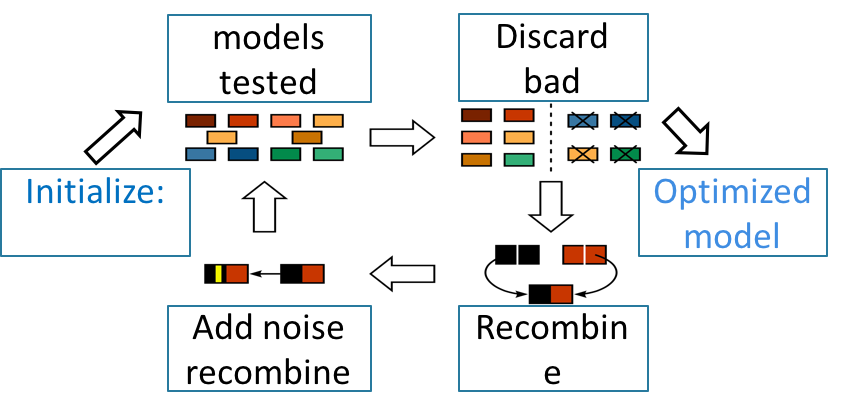
\includegraphics[width=0.7\linewidth]{figures/How_Genetic_Alg_Works.png}
  \caption{Genetic Algorithm Overview}
  \label{fig:GeneticAlgOver}
\end{figure}
  
\end{center}

In \ref{fig:GeneticAlgOver} I illustrate how a Genetic Algorithm (GA) generally works. The GA's evolution is guided by the application of selective pressure to iterative and refined sampling of the solution space.

\subsection{Significance}
% I wouldn't call this section "Significance".  In general, think of these sections as small modules that can be reshuffled and rearranged as needed.  You don't want to pin yourself to describing everything that is "Significant" right here.  In particular, you could call this section "Neuronal diversity".
Beyond experimental error, it is common to observe large variations in measurements of a single electrophysiological entity from neurons of the same classification. As an example, consider that measurements of neuron membrane input resistance may be different when recorded from different samples of the same neuron type. This variation is an essential consideration when evaluating the scientific merit of a computational model of a neuron-type. In this work, we propose to perform a large-scale analysis of model against data agreement and model against model agreement to expose the variation in biophysically realistic neuron models and cortical data. By analyzing the variance in data and among models and linking the variation to specific features and mechanisms, we also will better understand the heterogeneity of experimental measurements from a particular neuron-type. Performing a meta-analysis with a large number of models will provide other insights. We will determine whether there is higher variance in modeled electrical properties versus experimental neurophysiological measurements. We will examine whether an extensive collection of cortical models behaves more similarly to each other than to the data and will answer the question: does the space of all existing single cell models accurately represent the variability in experimental data?
Similarly, variation in the behavior of cortical neuronal networks is not well quantified. Tremendous research effort has been consumed producing several high-quality, experimentally informed cortical network models. Before creating another elaborate network model, we will determine whether these pre-existing approaches lead to networks with significantly different dynamic properties. Also, we will create an infrastructure that allows scientists to quantify the similarities and differences among networks and their dynamics – both biological and in silico.\newline
\newline
% Shouldn't this be a new section, about data integration?
Existing data sets are incomplete, consisting of a sparse sampling of cells in the rodent brain. By necessity, models are constrained using these incomplete data sets, leading to compensatory model development that synthesizes missing information. Missing data occurs at multiple levels during network construction including exact neuron to neuron wiring patterns, un-sampled morphologies, unknown synapse activation times, and unknown axon and dendrite synapse locations. Published models should not be regarded as final, but to improve models, it is vital that they are validated against newly-obtained experimental data. The proposed work will facilitate ongoing validation of biophysically realistic models. 
\\
% And this can go up into the section about diversity
Some electrophysiology data are challenging to integrate into existing models.
These include data collected from animal species that are not widely used in models such as marmoset, guinea pig, and even humans. 
Additionally, neuron-type data may come from a human, but the tissue samples may have been extracted from brain tissue in a pathological condition, such as eplipsey or alzheimers disease.
\\
In practice, open access data is not always useable, as it be derived from multiple species, multiple brain regions and different states of health. We will obtain a better understanding of region-dependent differences and species-dependent differences in order to help researchers map models onto a standardized rodent electrophysiological phenotype space.\\
\\
\subsection{Distinction of Optimization Approach From Other Approaches}
% This can be a fusion of your sections about multiobjective optimization, unit testing, and data integration (or whatever set of background items you think is fundamental to understanding the novelty of the work you have done).
Please elaborate on these limitations in a section called 



\subsection{Distinction of Large Scale Ananlysis From Other Approaches}
The large-scale meta-analysis described here has not been performed previously. For the first time, a large number of cortical neuron and neuronal network models are available in the standardized NeuroML format. Although the Allen Institute for Brain Science modeling project and the Blue Brain project both rigorously analyzed their single cell models, to the best of my knowledge there has not been an overarching meta-analysis across different cell and network model sources.\\
\\
Similarly, numerous modeling efforts have employed data-driven testing in model development workflows, but all these efforts have been based on non-standard ‘in-house’ model types and execution environments. In contrast, this work proposes to expand a pre-existing standardized model testing space, NeuronUnit, that supports model validation and re-use regardless of the model source. To date various NeuronUnit tests of action potential shape, electrical properties, and single cell morphologies exist; yet these tools are not unified. Some tests of network dynamics also currently exist; however, these tests are not integrated into a unified multiscale workflow. Although the work I describe only concerns single cell models in isolation, significantly, a unified workflow for exploring model data agreement would better locate errors in network behavior which are manifest at the network level but are caused by neuron-type models. \newline
\newline

% Add a section about model databases and the opportunities they will make available to you.  Describe how we don't really know whether the models in these databases match the experimental data they claim to recapitulate.  Describe some of the specific challenges in using "in house" data.
All of Intro should be chapter 1
1.1
1.2...

We built faster python implementations of two neuronal models (Izhi model and adaptive Exponential model). One of the implementations was based on MATLAB forward euler implementation of the Izhi model, another implementation of the Adaptive Exponential model came from vectorized python code, which was relatively slow.

Because I was able to use a tool \cite(numba) enables In Time compilation(JIT) , both of these models perform faster than standard neuron simulator versions in brian2 and NEURON.
2.1

    

 \section{Model Implementations}   

A constant error warning plagued brian2 investmentallations
\begin{verbatim}
Brian2 causes error:
 ERROR      Brian 2 encountered an unexpected error. If you think this is bug in Brian 2, please report this issue either to the mailing list at <http://groups.google.com/group/brian-development/>, or to the issue tracker at <https://github.com/brian-team/brian2/issues>. Please include this file with debug information in your report: /tmp/brian_debug_t0acbm4l.log  Additionally, you can also include a copy of the script that was run, available at: /tmp/brian_script_juzhsbph.py Thanks! [brian2]
Traceback (most recent call last):
\end{verbatim}

To make optimization of models tractable it was important to do ongoing feasibility testing. For example its important to evaluate the the utility of established model implementations, as using these models to optimize may not in fact be feasible.\\ 
\\
Despite an a large number of choices of FOSS reduced model
implementations, many off the shelf implementations were not useful, or significant intervention was required to make some established implementations workable inside an optimization framework. \\
\\
In two classes of model a feasible choice of implementation did not exist and it was easier to re-implement those models. The two models I re-implemented were
the Adaptive Exponential Integrate and fire Model, and also the IZHI
model.  In the work below, I profile existing model implementations, and
justify the reasons for re-implementing.\\
\\
This is in contrast to the brian2/neuraldynamics AdExp model, which took
between 2 or 3 times longer to find a rheobase current injection value. However the slowness is not caused by the simulation backend (brian2 which is relatively fast and efficient). The slow down is caused by the way the model is defined. Specifically the
model is defined in a middle code layer neurodynamics\cite{gerstner2014neuronal}.\\
\\
It is very likely, that the model implementation is correct, since Gerstner is an author of one of the original adaptive exponential publications, and the neural dynamics book that the brian2 code is strongly affiliated with. Since Integrate and Fire models don't formally include spikes when an implementation does include spikes, it is an optional add on.\\
\\
The AdExp neurodynamics models default implementation causes spikes with peaks below $0mV$, since the IZHI model like all integrate and fire models do not explicitly include spikes\\
\\
This is not technically wrong, but it violates
assumptions in the \emph{NeuronUnit} feature extraction protocol. The default spiking behavior, looks odd, and it is simply this poor model definition that is causing a slower optimizer performance. The optimizer takes an unusual waveform shape, and searches for longer in distant
parameter regions to find a good fit.\\
\\
Over the course of evaluating the brian neural dynamics model \cite{gerstner2014neuronal}. I experienced some phenomena that only occurred in the context of genetic algorithm optimization. The reason why optimization provides a different evaluation context is because, in optimization simulation objects are required to be created and destroyed rapidly and on mass. Brian2 is designed to be an efficient network simulator, the case of being designed for network simulation, may assume you will want to create a lot of neural models that persist efficiently together in memory (this was also a problem with PyNN models). Therefore you might see below, that while only one brian model exists in memory, performance is okay, but when creating and destroying models rapidly and on mass a slow down occurs.\\
\\
Below I have implemented a python integrator for the Adaptive
Exponential Integrate and fire model. This solver lead to faster
evaluations of current injection experiments. The integrator I developed
had a $0mV$ spiked when evaluated at default
parameter values.\\


Brian2 and sciunits sometimes collided in name space, and logging.
%\href{https://github.com/scidash/sciunit/pull/124/files/83907ba68740642178ebb91084f6e382e06a43c4#diff-d68791d2ed5dfaa96a900be6180bd950}

\section{Profiling the JIT enabled AdExp Model}
Mean time taken on single model evaluation:$ 0.0012554397583007812s $
Mean time taken to compute rheobase:
$0.183s $


Even faster than Izhikevich implementation which was: $ 0.462s $ $  0.002 s$
Rheobase takes a mean of 15 model evaluations.
\begin{figure}    
\begin{center}
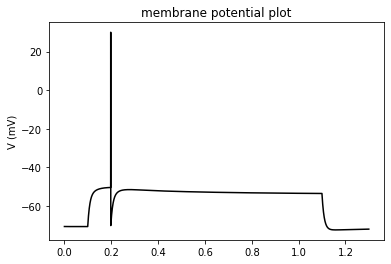
\includegraphics[width=0.25\linewidth]{figures/backend_check_files/backend_check_6_2.png}
\caption{}

\end{center}
\end{figure}

%\begin{verbatim}
%    251 ms +- 5.02 ms per loop (mean +- std. dev. of 2 runs, 1 loop each)
%    240 ms +- 11.1 ms per loop (mean +- std. dev. of 2 runs, 1 loop each)
%    223 ms +- 12.5 ms per loop (mean +- std. dev. of 2 runs, 1 loop each)
%\end{verbatim}

\begin{verbatim}
    922 ms +- 12.7 ms per loop (mean +- std. dev. of 7 runs, 1 loop each)
\end{verbatim}

\subsection{Compare parallel to serial speeds, and accuracy}

Below is the Brian2/NeuralDynamics AdExp model. In-order to make the spike height greater than $0mV$ it was easier to use computer code to schedule waveform modifications that occur straight after the the brian2 simulation, these scheduled waveform modifications can be considered part of a peripheral shell of simulation code. In postprocessing
the waveform data type is a Neo Wave form object that is artificially the algorithm of determining rheobase and displaying results. The time of this model is determined on multiple factors, as discussed elsewhere, execution time is not uniform across model parameterizations. Models with multispiking behavior will take longer to solve.

Simulation times for this model vary, dramatically possibly because of
lazy evaluation, the simulation times may vary according to what else
you are running on your computer. Not all models experience a speed up when executed in parallel, however
this model was faster in the parallel Rheobase determination algorithm. Some common times are: $3.92,6.75,4.48,5.17$. Mean time was:

\subsection{Comparison of Times Taken to Find Rheobase}
Custom implementation JIT enabled implementation: $4.0s$. 
Brian2 taken to find Rheobase: $4.40s$ (serial), $3.976s$ (parallel).

The evaluation times between Brian2 and the custom written
integrator are similar. Both have average rheobase solution times of approximately 4 seconds, however the spike shape derived from the custom written integrator look more realistic under default paramaterizations. The biological plausibility of default model paramaterization has consequences for model optimization speed, because when  models undergo mutation and cross-over the mean of random models regressors towards the default model initialization, and if the default model is a bad fit to data, the average model sampled by the genetic algorithm will also be bad to data.\\

\begin{center}
\begin{figure}
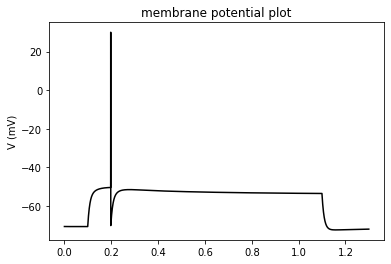
\includegraphics{figures/backend_check_files/backend_check_4_2}
\caption{Default model parameterization of the custom written integrator}
\end{figure}
\end{center}


\begin{center}
\begin{figure}

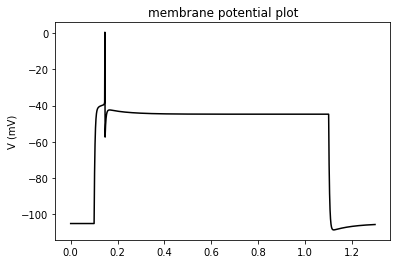
\includegraphics{figures/backend_check_files/backend_check_12_10}
\caption{Model parameterization of the brian2 simulator with the customization: interpolated spike height, forced to be above $0mV$}
\end{figure}

\end{center}
    
\begin{verbatim}
    272 ms +- 66.5 $/mu$s per loop (mean +- std. dev. of 2 runs, 1 loop each)
\end{verbatim}

The next model to be evaluated is the NEURON Izhi model. The NEURON Izhi model has various draw backs. 1. It depends on an external file which must be recompiled each time this project is recreated. 2. The build environment of NEURON is non-trivial, and only a super dedicated NEURON modeller would install it on their system. Any performance advantage of using NEURON investment does not exceed the installation cost of installing the program. 3. The model implementation code is less generalizable than than the published Izhi model itself. Where the standard NEURON-NeuroML code only covers the Regular-Spiking model * This is likely due to a name space conflict between Capacitance. Neuron has a `capacitive' mechanism inside modelled Neurons, this particular model has section capacitance as well as an introduced capacitive term inside a C-compiled mechanism. Both contribute to a the membrane
potential calculation. * The NEURON Izhi model took $78$ seconds to find the rheobase current injection value $ 51.79367065 * pA $.

    
%\begin{center}
 %   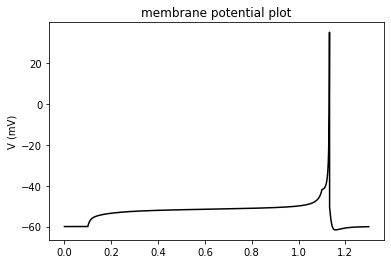
\includegraphics[width=0.7\textwidth,]{chapters/figures/backend_check_files/backend_check_14_2.png}
%    \caption{where is picture}
%\end{center}


%\begin{figure}
%    \centering
%    \includegraphics{chapters/normal_distribution}
%    \caption{This is your image%}
%    \label{fig:my_label}
%\end{figure}



% https://www.overleaf.com/learn/how-to/Images_not_showing_up 
        
The forward Euler python IZhi model is very fast. The forward euler
implementation utilized Numba JIT. Rheobase is found in under a second,
and in many cases close 0.5 seconds. This represents a very dramatic
speed up. Unlike the NEURON NeuroML implementation of the izhikitich equation,
this implementation is just as generalizable as the original MATLAB
implementation of the izhikitich model.


\begin{verbatim}
  time taken on
  block 0.6859951019287109 \textbackslash{}n3.3 ms +- 9.79 $\mu$s per loop (mean +- std. dev. of 2
  runs, 100 loops each)\textbackslash{}n3.32 ms +- 30.9 us per loop (mean +- std. dev. of 2 runs,
  100 loops each)\textbackslash{}n3.19 ms +- 10.9 us per loop (mean +- std. dev. of 2 runs, 100

\end{verbatim}
        
\section{Python/LEMS and NEURON versions of single compartment Conducance Model.}

Conductance based models took approximately the same amount of
time to evaluate the Rheobase search algorithm as the python
implementation.

%This problem in the default parameterization of the python model was later located in the scale or units of capacitance, if default capacitance parameterization is multiplied by 100.0 the problem goes away.

time taken on block $ 12.6s $

\begin{center}
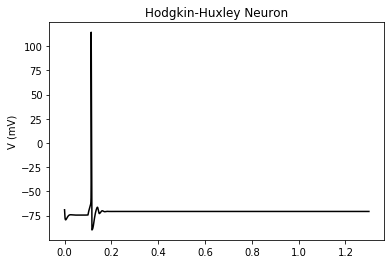
\includegraphics{figures/backend_check_files/backend_check_22_2}
\end{center}

$ 1.40762329 * pA $


\subsection{NEURON versions of single compartment Conducance
model.}

Hodgkin Huxley Conductance based channels models took approximately the same amount of time to evaluate the Rheobase search algorithm as the python implementation.

%The NEURON implementation was slightly faster, and the default parameterization of the model lacked `ringing'', or below threshold oscillations that the Python ODE version had under default conditions.

%This problem in the default parameterization of the python model was later located in the scale or units of capacitance, if default capacitance parameterization is multiplied by 100.0 the problem goes away.

    \begin{verbatim}
time taken on block 8.573923826217651
    \end{verbatim}


    %\graphicspath{ {../figures/} }
    \begin{center}
    \begin{figure}
    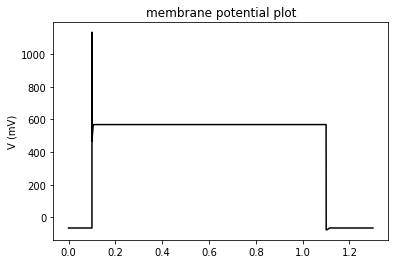
\includegraphics{figures/backend_check_files/backend_check_26_2}
    %kend_check_files/backend_check_26_2.png}
    \end{figure}
    
    \end{center}
\begin{verbatim}
112.5 pA
'value': array(1.40645904) * pA
\end{verbatim}


\begin{verbatim}
\{'El\_reference': -0.07016548013687134, 'C': 3.990452661875942e-10,
'init\_threshold': 0.02964956889477108, 'th\_inf': 0.02964956889477108,
'spike\_cut\_length': 109.5, 'init\_voltage': -35.0, 'R\_input': 910258965.9792937\}
time taken on block 0.23476457595825195
\end{verbatim}

    


$ 112.5 pA $
$0.0 mV$ $-0.065 mV$

    \begin{verbatim}
    \{'value': array(183.33333333) * pA\}
    \end{verbatim}

\begin{verbatim}
array(112.5) * pA
\end{verbatim}


\begin{verbatim}
    0.017240506310425608 mV -0.08583939747094235 mV
    0.017240506310425608 mV -0.08583939747094235 mV
\end{verbatim}

    \begin{center}
    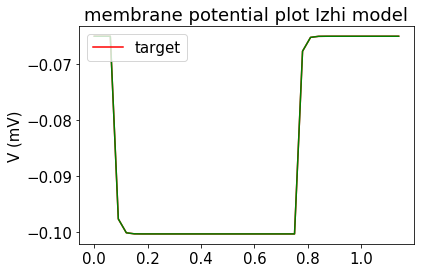
\includegraphics{figures/backend_check_files/backend_check_32_2.png}
    \end{center}

2.2
\section*{Technical Details of the Optimizer}
\begin{itemize}

\item Experimental Recording Features from Neuroelectro. And some from the Allen SDK.
\item The algorithms IBEA and NSGA2 seem to result in similar optimization convergence speeds, and similar solution quality.

%\item Python, NeuroUnit, 

\subsetion{Model/Test combinations}

Contrast with other optimization approaches:


There are two different strategies, one strategy involves evaluating goodness of fit, only at one current injection strength for every gene. Another approach is a bit more generous, in that, rather than allowing models to instantly fail to evoke a spike at the appropriate current injection, that models specific rheobase value is found, and all other tests are evaluated at the current injection value. The consequence of accomodating poorer fits on the Rheobase test, is allows models to compete on the other seven or more different fitness criteria.

\subsection{Elephant Test Suite}
At a count of eight tests (five useable) the elephant derived suite was relatively compact. The elephant tests suite is concerned with core ephysiology measurements, the particular measurements chosen were important because, for example capacitance, and input resistance directly affect the evolution of reduced model governing equations. Taken as a collection these ephysiological properties as a collection also determine spiking waveform shape. 

Capacitance, Rheobase, Time Constant, Input Resistance, Resting Potential

\item Result It when models were fitted using the following measurements alone, the resulting models were also fitted to spike half-width, arguably because the membrane time-constant, and membrane capacitance together encode spike-half width.

\subsection{Electrophysiology Feature Extraction Library}

Many of the EFEL measurements, and Allen SDK Feature measurements pertain to spike train statistics, because model fitting to spike train statistics is a productive and well understood domain, we did not utilize spike train statistics in model fitting. Instead EFEL spike shape and electrophysiology measurements were applied.\\
\\
Through trial and error experimentation the following EFEL features were demonstrated to result in helpfull and tractible error surfaces. In simulated constraint paradigms using the aforementioned EFEL fitness criteria, lead to recovery of optimal models. This finding did not apply to the entire collection of EFEL features however.\\
\\
In a large scale analysis of variance between models and data see section large_scale_variance

\href{run:./RESULTS_large_scale_variance.tex}{RESULTS_large_scale_variance.tex}



'AHP_depth_abs_3.0x','sag_ratio2_3.0x','ohmic_input_resistance_1.5x','sag_ratio2_1.5x','peak_voltage_3.0x','peak_voltage_1.5x','voltage_base_3.0x','voltage_base_1.5x','Spikecount_1.5x','Spikecount_3.0x','ohmic_input_resistance_vb_ssse_1.5x'


\item Unlike in BluePyOpt \cite{Werner} and Allen Institute optimization workflows \cite{gouwens} rheobase current injection was applied is a soft constraint. 

However, this work differs from other work in that rheobase current injection was found for every different model paramerisation.\\
\\
\item Rheobase value as a soft constraint. This means that current injection values are a variable model parameter. The exact value of current used is determined via exploring the model response to current injections of varying amplitude. The exact value, its value is determined by other model parameters.

\item spike shape measurements and error functions. We used a set of 8 different experimental measurements NeuronUnit.
\end{itemize}


\begin{figure}
	\includegraphics[width=\maxwidth{\textwidth}]{figures/normal_distribution.png}
    \caption{Error functions were evaluated with the assistance of a library: \emph{NeuronUnit} 
    were based on finding a normal distribution on electro physiology measurements, 
    and then measuring model outputs and mapping the model behavior onto
     a place on the experimental normal distribution. Scores that where closer to the
      experimental mean where deemed to be low in error.
	Z-scores obtained via NeuronUnit can be thought of as  }
	\label{figure\arabic{figurecounter}}
	
\caption{Caption}
	
\end{figure}

2.3
Here I show graphs of


In a simulated experiment, existing models were instantiated using a randomly chosen model parameters.

<!--The reason for this exercise is-->

In the class of reduced neural models we are optimizing, are not arbitrary waveform generators. The models have intrinsic restrictions that prevent them from matching perfectly with experimental waveforms.

When constraints are derived from model measurements, intrinsic model restrictions no longer apply. Optimized models should match perfectly with the simulated experiments. 

* Failure to match is indicative of three things:
- Optimizer code design failure
- Conceptual Failure
- Failure to setup tractable optimization problems.
- When inverting linear equations, finding a unique solution requires that the number of constraining equations is greater than the number of free variables you are solving for:

\section{Verification}
It was important to be able to create a ground truths that were always possible for the optimizer to match exactly. Often experimental data implies waveform shapes that are beyond the capabilities of the model that is to be fitted. Simulating experimental measurements meant, that model limitations can be understood separately from optimizer limitations.

\section{Optimizer Limitations}
\begin{itemize}
    \item 
\item  N free model parameters << N_constraints
\item  In our specific design this expands to:
\item  (model parameters + current_value parameter) << N (indipendent and uncorrelated) constraints.
\item  
For the different classes of Reduced Model we show that 
\end{itemize}
\end{item}

2.4

    

 \section{Model Implementations}   

A constant error warning plagued brian2 investmentallations
\begin{verbatim}
Brian2 causes error:
 ERROR      Brian 2 encountered an unexpected error. If you think this is bug in Brian 2, please report this issue either to the mailing list at <http://groups.google.com/group/brian-development/>, or to the issue tracker at <https://github.com/brian-team/brian2/issues>. Please include this file with debug information in your report: /tmp/brian_debug_t0acbm4l.log  Additionally, you can also include a copy of the script that was run, available at: /tmp/brian_script_juzhsbph.py Thanks! [brian2]
Traceback (most recent call last):
\end{verbatim}

To make optimization of models tractable it was important to do ongoing feasibility testing. For example its important to evaluate the the utility of established model implementations, as using these models to optimize may not in fact be feasible.\\ 
\\
Despite an a large number of choices of FOSS reduced model
implementations, many off the shelf implementations were not useful, or significant intervention was required to make some established implementations workable inside an optimization framework. \\
\\
In two classes of model a feasible choice of implementation did not exist and it was easier to re-implement those models. The two models I re-implemented were
the Adaptive Exponential Integrate and fire Model, and also the IZHI
model.  In the work below, I profile existing model implementations, and
justify the reasons for re-implementing.\\
\\
This is in contrast to the brian2/neuraldynamics AdExp model, which took
between 2 or 3 times longer to find a rheobase current injection value. However the slowness is not caused by the simulation backend (brian2 which is relatively fast and efficient). The slow down is caused by the way the model is defined. Specifically the
model is defined in a middle code layer neurodynamics\cite{gerstner2014neuronal}.\\
\\
It is very likely, that the model implementation is correct, since Gerstner is an author of one of the original adaptive exponential publications, and the neural dynamics book that the brian2 code is strongly affiliated with. Since Integrate and Fire models don't formally include spikes when an implementation does include spikes, it is an optional add on.\\
\\
The AdExp neurodynamics models default implementation causes spikes with peaks below $0mV$, since the IZHI model like all integrate and fire models do not explicitly include spikes\\
\\
This is not technically wrong, but it violates
assumptions in the \emph{NeuronUnit} feature extraction protocol. The default spiking behavior, looks odd, and it is simply this poor model definition that is causing a slower optimizer performance. The optimizer takes an unusual waveform shape, and searches for longer in distant
parameter regions to find a good fit.\\
\\
Over the course of evaluating the brian neural dynamics model \cite{gerstner2014neuronal}. I experienced some phenomena that only occurred in the context of genetic algorithm optimization. The reason why optimization provides a different evaluation context is because, in optimization simulation objects are required to be created and destroyed rapidly and on mass. Brian2 is designed to be an efficient network simulator, the case of being designed for network simulation, may assume you will want to create a lot of neural models that persist efficiently together in memory (this was also a problem with PyNN models). Therefore you might see below, that while only one brian model exists in memory, performance is okay, but when creating and destroying models rapidly and on mass a slow down occurs.\\
\\
Below I have implemented a python integrator for the Adaptive
Exponential Integrate and fire model. This solver lead to faster
evaluations of current injection experiments. The integrator I developed
had a $0mV$ spiked when evaluated at default
parameter values.\\


Brian2 and sciunits sometimes collided in name space, and logging.
%\href{https://github.com/scidash/sciunit/pull/124/files/83907ba68740642178ebb91084f6e382e06a43c4#diff-d68791d2ed5dfaa96a900be6180bd950}

\section{Profiling the JIT enabled AdExp Model}
Mean time taken on single model evaluation:$ 0.0012554397583007812s $
Mean time taken to compute rheobase:
$0.183s $


Even faster than Izhikevich implementation which was: $ 0.462s $ $  0.002 s$
Rheobase takes a mean of 15 model evaluations.
\begin{figure}    
\begin{center}
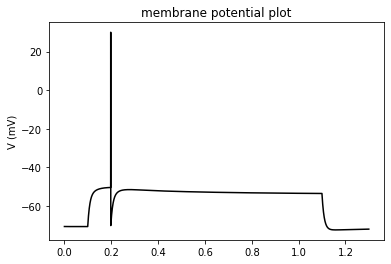
\includegraphics[width=0.25\linewidth]{figures/backend_check_files/backend_check_6_2.png}
\caption{}

\end{center}
\end{figure}

%\begin{verbatim}
%    251 ms +- 5.02 ms per loop (mean +- std. dev. of 2 runs, 1 loop each)
%    240 ms +- 11.1 ms per loop (mean +- std. dev. of 2 runs, 1 loop each)
%    223 ms +- 12.5 ms per loop (mean +- std. dev. of 2 runs, 1 loop each)
%\end{verbatim}

\begin{verbatim}
    922 ms +- 12.7 ms per loop (mean +- std. dev. of 7 runs, 1 loop each)
\end{verbatim}

\subsection{Compare parallel to serial speeds, and accuracy}

Below is the Brian2/NeuralDynamics AdExp model. In-order to make the spike height greater than $0mV$ it was easier to use computer code to schedule waveform modifications that occur straight after the the brian2 simulation, these scheduled waveform modifications can be considered part of a peripheral shell of simulation code. In postprocessing
the waveform data type is a Neo Wave form object that is artificially the algorithm of determining rheobase and displaying results. The time of this model is determined on multiple factors, as discussed elsewhere, execution time is not uniform across model parameterizations. Models with multispiking behavior will take longer to solve.

Simulation times for this model vary, dramatically possibly because of
lazy evaluation, the simulation times may vary according to what else
you are running on your computer. Not all models experience a speed up when executed in parallel, however
this model was faster in the parallel Rheobase determination algorithm. Some common times are: $3.92,6.75,4.48,5.17$. Mean time was:

\subsection{Comparison of Times Taken to Find Rheobase}
Custom implementation JIT enabled implementation: $4.0s$. 
Brian2 taken to find Rheobase: $4.40s$ (serial), $3.976s$ (parallel).

The evaluation times between Brian2 and the custom written
integrator are similar. Both have average rheobase solution times of approximately 4 seconds, however the spike shape derived from the custom written integrator look more realistic under default paramaterizations. The biological plausibility of default model paramaterization has consequences for model optimization speed, because when  models undergo mutation and cross-over the mean of random models regressors towards the default model initialization, and if the default model is a bad fit to data, the average model sampled by the genetic algorithm will also be bad to data.\\

\begin{center}
\begin{figure}
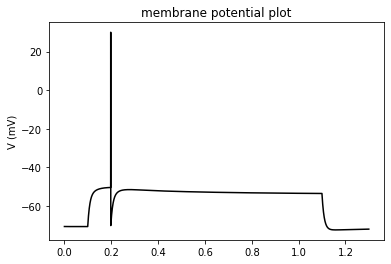
\includegraphics{figures/backend_check_files/backend_check_4_2}
\caption{Default model parameterization of the custom written integrator}
\end{figure}
\end{center}


\begin{center}
\begin{figure}

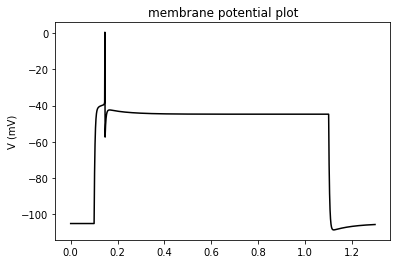
\includegraphics{figures/backend_check_files/backend_check_12_10}
\caption{Model parameterization of the brian2 simulator with the customization: interpolated spike height, forced to be above $0mV$}
\end{figure}

\end{center}
    
\begin{verbatim}
    272 ms +- 66.5 $/mu$s per loop (mean +- std. dev. of 2 runs, 1 loop each)
\end{verbatim}

The next model to be evaluated is the NEURON Izhi model. The NEURON Izhi model has various draw backs. 1. It depends on an external file which must be recompiled each time this project is recreated. 2. The build environment of NEURON is non-trivial, and only a super dedicated NEURON modeller would install it on their system. Any performance advantage of using NEURON investment does not exceed the installation cost of installing the program. 3. The model implementation code is less generalizable than than the published Izhi model itself. Where the standard NEURON-NeuroML code only covers the Regular-Spiking model * This is likely due to a name space conflict between Capacitance. Neuron has a `capacitive' mechanism inside modelled Neurons, this particular model has section capacitance as well as an introduced capacitive term inside a C-compiled mechanism. Both contribute to a the membrane
potential calculation. * The NEURON Izhi model took $78$ seconds to find the rheobase current injection value $ 51.79367065 * pA $.

    
%\begin{center}
 %   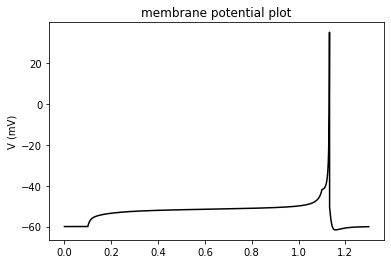
\includegraphics[width=0.7\textwidth,]{chapters/figures/backend_check_files/backend_check_14_2.png}
%    \caption{where is picture}
%\end{center}


%\begin{figure}
%    \centering
%    \includegraphics{chapters/normal_distribution}
%    \caption{This is your image%}
%    \label{fig:my_label}
%\end{figure}



% https://www.overleaf.com/learn/how-to/Images_not_showing_up 
        
The forward Euler python IZhi model is very fast. The forward euler
implementation utilized Numba JIT. Rheobase is found in under a second,
and in many cases close 0.5 seconds. This represents a very dramatic
speed up. Unlike the NEURON NeuroML implementation of the izhikitich equation,
this implementation is just as generalizable as the original MATLAB
implementation of the izhikitich model.


\begin{verbatim}
  time taken on
  block 0.6859951019287109 \textbackslash{}n3.3 ms +- 9.79 $\mu$s per loop (mean +- std. dev. of 2
  runs, 100 loops each)\textbackslash{}n3.32 ms +- 30.9 us per loop (mean +- std. dev. of 2 runs,
  100 loops each)\textbackslash{}n3.19 ms +- 10.9 us per loop (mean +- std. dev. of 2 runs, 100

\end{verbatim}
        
\section{Python/LEMS and NEURON versions of single compartment Conducance Model.}

Conductance based models took approximately the same amount of
time to evaluate the Rheobase search algorithm as the python
implementation.

%This problem in the default parameterization of the python model was later located in the scale or units of capacitance, if default capacitance parameterization is multiplied by 100.0 the problem goes away.

time taken on block $ 12.6s $

\begin{center}
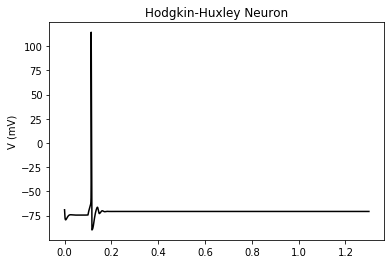
\includegraphics{figures/backend_check_files/backend_check_22_2}
\end{center}

$ 1.40762329 * pA $


\subsection{NEURON versions of single compartment Conducance
model.}

Hodgkin Huxley Conductance based channels models took approximately the same amount of time to evaluate the Rheobase search algorithm as the python implementation.

%The NEURON implementation was slightly faster, and the default parameterization of the model lacked `ringing'', or below threshold oscillations that the Python ODE version had under default conditions.

%This problem in the default parameterization of the python model was later located in the scale or units of capacitance, if default capacitance parameterization is multiplied by 100.0 the problem goes away.

    \begin{verbatim}
time taken on block 8.573923826217651
    \end{verbatim}


    %\graphicspath{ {../figures/} }
    \begin{center}
    \begin{figure}
    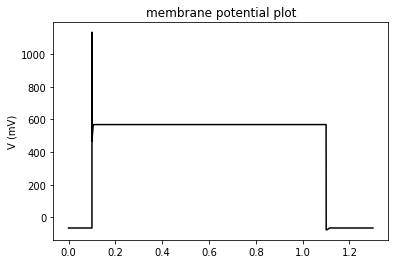
\includegraphics{figures/backend_check_files/backend_check_26_2}
    %kend_check_files/backend_check_26_2.png}
    \end{figure}
    
    \end{center}
\begin{verbatim}
112.5 pA
'value': array(1.40645904) * pA
\end{verbatim}


\begin{verbatim}
\{'El\_reference': -0.07016548013687134, 'C': 3.990452661875942e-10,
'init\_threshold': 0.02964956889477108, 'th\_inf': 0.02964956889477108,
'spike\_cut\_length': 109.5, 'init\_voltage': -35.0, 'R\_input': 910258965.9792937\}
time taken on block 0.23476457595825195
\end{verbatim}

    


$ 112.5 pA $
$0.0 mV$ $-0.065 mV$

    \begin{verbatim}
    \{'value': array(183.33333333) * pA\}
    \end{verbatim}

\begin{verbatim}
array(112.5) * pA
\end{verbatim}


\begin{verbatim}
    0.017240506310425608 mV -0.08583939747094235 mV
    0.017240506310425608 mV -0.08583939747094235 mV
\end{verbatim}

    \begin{center}
    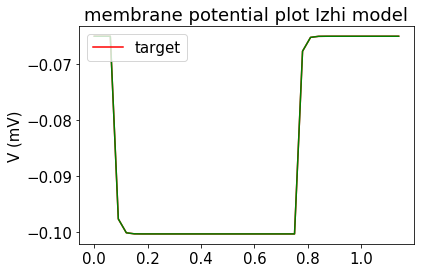
\includegraphics{figures/backend_check_files/backend_check_32_2.png}
    \end{center}

Section 3
Results
3.1





Four factors needed to be controlled for, before we locate the cause of poor model/experiment fits. Those factors were: the informativeness of measurement errors, the performance of the optimizer, data quality, and model quality.

The digital models we used were known to be not flexible enough to match all electrical features from cell experiments all the time; these models are by nature, self-constrained and therefore they cannot to be fitted to all experimental waveforms. Additionally the data sources may also have some fidelity problems, it was necessary to create data source independent "ground truths", by synthesising plausible data, with the digital models, and optimizing against these ground truths. Because the DEAP genetic algorithm, has been shown to be able solve Rastrigrins function, we expect that our derivative frame work, should be able to fit to simulated data sources, with a high degree of precision, and that is what we found.


The optimizer was capable of producing perfect fits under ideal circumstances. We showed that the measurements the genetic algorithm was using were able to act as informative guides. Since we are confident about the optimizers ability to fit to synthesized data we can then locate sources of model/data disagreement in other places. \\ 
In the subsequent tables and figures when the measurements:time constant, capacitance, Rheobase, Resting potential and Input resistance are used to constrain optimization.
\begin{figure}
    \centering
    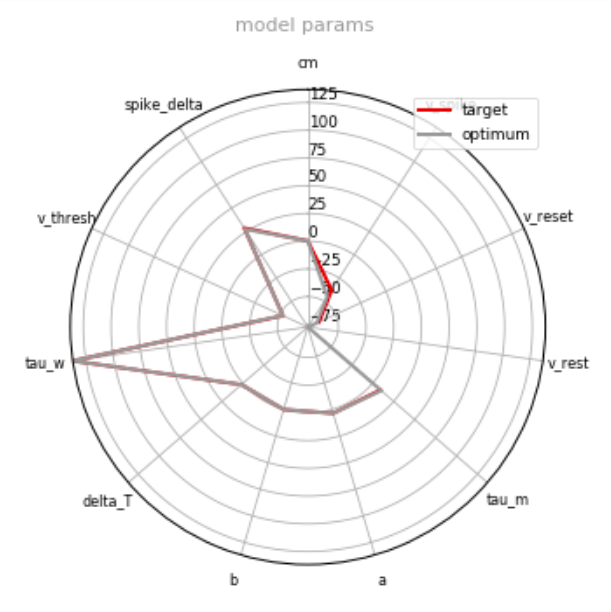
\includegraphics{figures/radar_coordinates.png}
    \caption{This radar plot of model parameters, reveals two mutually inclusive sets, both model parameter values 1 randomly selected, 2 found by the optimizer closely match.}
    \label{fig:my_label}
\end{figure}


%coincide 
\begin{figure}
    \centering
    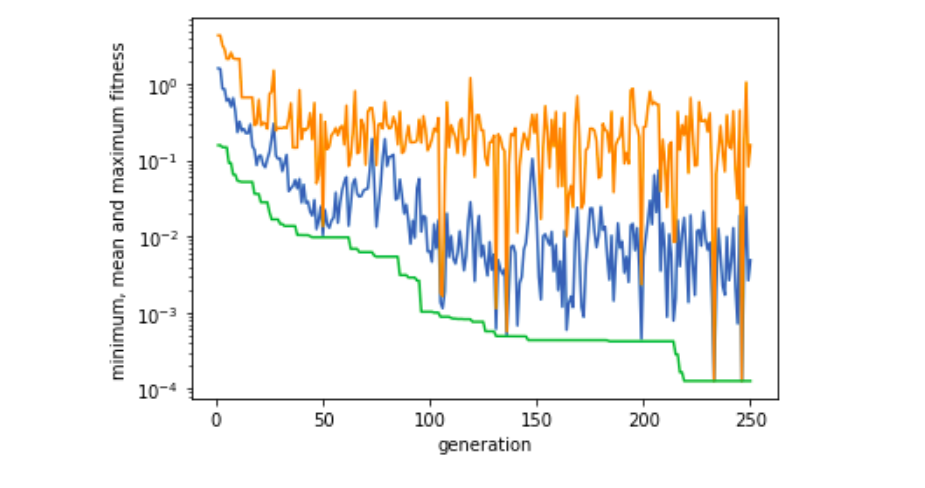
\includegraphics{figures/simulated_data_stats.png}
    \caption{Caption}
    \label{fig:my_label}
\end{figure}

\begin{figure}
    \centering
    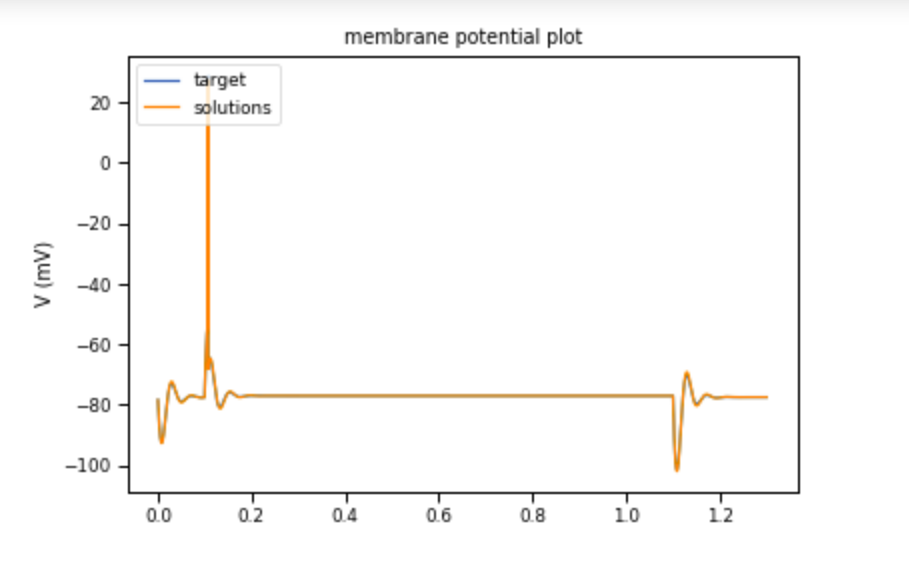
\includegraphics{figures/simulated_data_supra_threshold.png}
    \caption{Caption}
    \label{fig:my_label}
\end{figure}
\begin{figure}
    \centering
    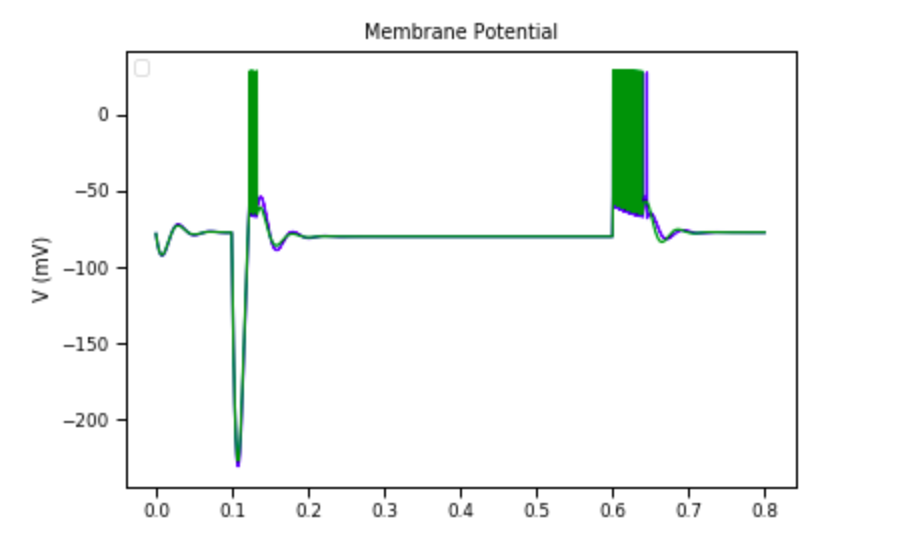
\includegraphics{figures/simulated_data_sub_threshold.png}
    \caption{Caption}
    \label{fig:my_label}
\end{figure}

\begin{figure}
    \centering
    \includegraphics[scale=0.7]{figures/sim}
    \caption{Optimizer evolution, green line tracks evolution of best fitness, blue line average fitness, orange line is worst fitness. GA params, $NGEN=200$, $MU=50$,$cxp=0.3$,$mupb=0.2$ from this plot can see that genes are storing and exploiting information, $cxp+mutpb=0.5$, so $50\%$ of genes are conserved between generations }
    \label{fig:my_label}
\end{figure}

\begin{figure}
    \centering
    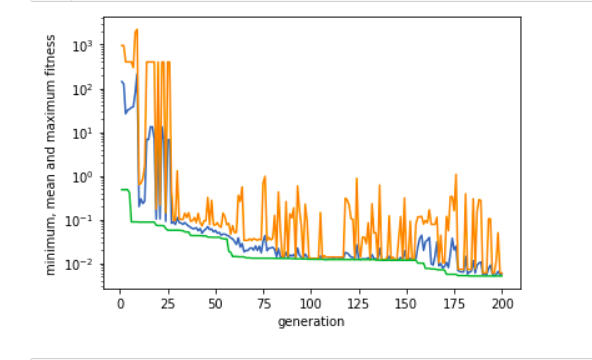
\includegraphics[scale=0.7]{figures/optimizer_internal_validation}
    \caption{Optimizer evolution, green line tracks evolution of best fitness, blue line average fitness, orange line is worst fitness. GA params, $NGEN=200$, $MU=50$,$cxp=0.3$,$mupb=0.2$ from this plot can see that genes are storing and exploiting information, $cxp+mutpb=0.5$, so $50\%$ of genes are conserved between generations }
    \label{fig:my_label}
\end{figure}


\begin{table}[ht]
\centering
\resizebox{\textwidth}{!}{
\begin{tabular}{llll}
\toprule
{} &    observations &     predictions & Z-Scores \\
\midrule
RheobaseTest         &         1.62 pA &         1.62 pA &        0 \\
TimeConstantTest     &        13.18 ms &        13.18 ms &        0 \\
RestingPotentialTest &       -77.43 mV &       -77.43 mV &        0 \\
InputResistanceTest  &  270.84 megaohm &  270.84 megaohm &        0 \\
CapacitanceTest      &        48.65 pF &        48.65 pF &        0 \\
FITest               &    [7.51 Hz/pA] &    [7.51 Hz/pA] &        0 \\
\bottomrule
\end{tabular}}
\end{table}

AP width, amplitude, and AP threshold errors, did not participate in guiding optimization, because as I have explained, those measurements are not objective between model instances, and thus they lead to misleading error measurements. These tables show that the optimizer can re-cover ground truths that are derived from simulated data. This result allows us to confidently argue that in fitted models, the cause of model/experiment disagreement must be located in either the data, or the models, but not the optimization process, or the choice of error signals which are demonstrably sound.

%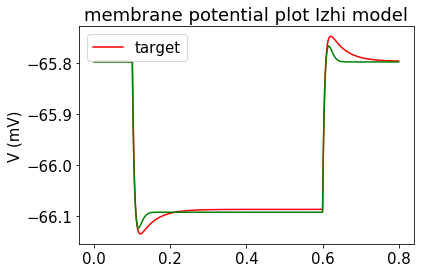
\includegraphics[]{figures/simulated_data_convergence_passive_fits.png}

\begin{figure}
    \begin{center}
    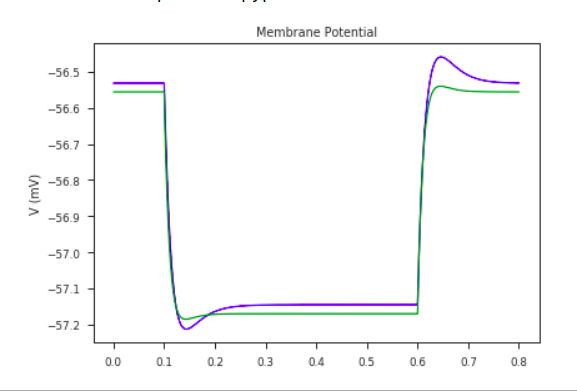
\includegraphics[scale=0.65]{figures/passive_model_agreement}
    \caption{Agreement between a simulated constraint waveform, and an optimized waveform, when both simulated constraint model and optimized model undergo a current injection value of $-10pA$}
    \end{center}
    \label{fig:my_label}
\end{figure}




The design of the optimizer used in this work, computed rheobase for each model, what that means is a new current is required to apply current injection tests to tests that are spiking in nature.\\
%In the optimizer design used here.

$N-free-model-parameters << N-constraints$
$(model parameters + current-injection-value-parameter) << N$ $(independent and uncorrelated)$ constraints.$

For the different classes of Reduced Model we show that the optimizer converges when data is simulated.

In a simulated experiment, existing models were instantiated using a randomly chosen model parameters.

In the class of reduced neural models we are optimizing, are not arbitrary waveform generators. The models have intrinsic restrictions that prevent them from matching perfectly with experimental waveforms.

When constraints are derived from model measurements, intrinsic model restrictions no longer apply. Optimized models should match perfectly with the simulated experiments. 

* Failure to match is indicative of: -- Failure to setup tractable optimization problems. Too higher a dimension.

- When inverting linear equations, finding a unique solution requires that the number of constraining equations is greater than the number of free variables you are solving for:

\section{Pitfalls}
Choosing optimizer constraints, that cause visible ripples in error surface.
To protect against a situation where the collection of error sources guiding optimization are too correlated with each other, to act as 


\section{Verification}
Ground truths are model solutions that we know are correct independently from the optimizer. One way to establish ground truths is to identify the global minima by exhaustively searching the solution space. An exhaustive search is a reasonable approach when you consider only one or two model parameters are free parameters, however if one does 100 samples in each of N dimensions then one must make samples $100^{N}$ total samples to be sure of ehaustively searching, assuming the most efficient code, hardware and development time $N=3$, may be the highs.  Also the choice of 100 samples is nominal, 100 samples could be either too fine or too sparse, depending on how if the parameter being searched exhibits 2nd order sensitivity.

It is more computationally efficient to obtain ground truths by simulating constraining data using digital models. It is easy to simulate constraining data, all that is required is that you take a neuronal model and measure its behavior in response to carefuly chosen current injection values. Measured behavior can then be used to construct NeuronUnit tests, were the measurements become "observations", or observed behaviors. To make the simulated data cover a range of circumstances, one can make different NU measurements by randomly choosing different parameter values of models to find.

It was important to be able to establish ground truths that were always possible for the optimizer to match exactly. Often experimental data implies waveform shapes that are beyond the capabilities of the model that is to be fitted. Simulating experimental measurements meant, that model limitations can be understood separately from optimizer limitations.


3.2
Chapter about (difficulty of) recovering averages of parameter sets for models
- Pick two different parameter sets, each of which can be easily recovered/verified independently
- Compute features for both, and average features together (like one would imagine is happening for neuroelectro data)
- Try to recover these averaged features (it could be hard/bad).
%Model repurposing is common and it is done on a network scale \cite{traub} and an individual cell scale.
%Experimental evidence is starting to reveal that model re-purposing of pyramidal neurons might not be a good idea.
It is known that neural models and experimental measurements diverge generally and in important ways, however, it is desirable to know the specific sources of divergence. Models and experiments may disagree, for two reasons: A the model is not flexible enough to satisfy a particular constraint simultaneously to a collection of constraints, or, B the model was incorrectly fitted to the wrong type of measurement (for example model fitted to spike times at the expense of Rheobase, and FISlope). 

Since we don't yet have complete knowledge of model/experiment divergence, we don't necessarily know the best features to target with regards to model fitting. Specific knowledge of model/data disagreement facilitates the prioritized selection of features that should guide optimization. 
%a voltage recordings should be prioritized as optimization constraints.



\begin{figure}
    \centering
    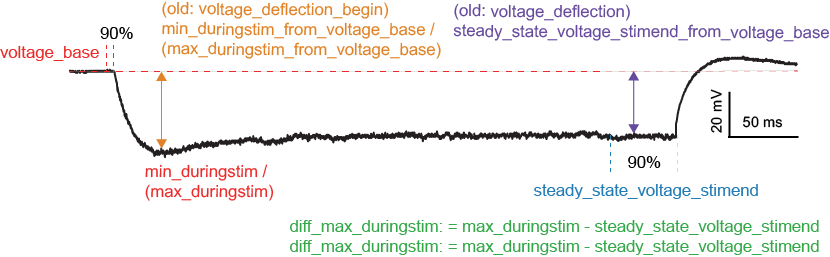
\includegraphics{figures/voltage_features.png}
    \caption{Caption}
    \label{fig:voltage_figures}
\end{figure}
\begin{figure}
    \centering
    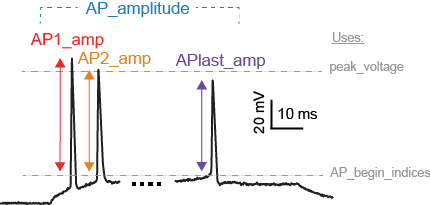
\includegraphics{figures/AP_Amplitude.png}
    \caption{Caption}
    \label{fig:features_example}
\end{figure}

\begin{figure}
    \centering
    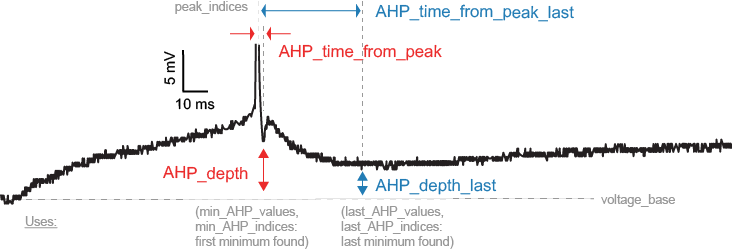
\includegraphics{figures/AHP.png}
    \caption{Caption}
    \label{fig:features_example_ahp}
\end{figure}



\subsubsection{Features} 
Consider a voltage recording at the location of the membrane of a neuron. Teams of researchers have already segmented voltage recordings into labelled sections, each section has a classification that is based on the shape of waveform in a limited region see figure \ref{fig:voltage_figures} for example. Rather than specifying by name each measurement it is often useful to refer collectively to these measurable shapes as "features". 

In the following multivariate analysis we analyze hundreds of such features, and we summarize important differences in a subset of this high dimensional feature space.  Below, I describe some neuronal model features that agreed well with experiments, and some features that diverged.


\subsubsection{Publications Associated with Model Sources}
972 models, 448 experiments.

Allen Institute for Brain Science Cell Types Database [7] can be accessed using the SDK. 

The Blue Brain Project Dataset can be obtained from the Data Navigator, or an API.

\begin{itemize}
\item Allen Institute V1 \cite{gouwens2018systematic}
\item Somatosensory Cortex \cite{markram2015} 
\end{itemize}

\subsubsection{Feature Extraction Libraries}
\begin{table}
\centering
%\resizebox{\textwidth}{!}{
\begin{tabular}{lll}
%\toprule
{} EFEL Ephys Feature Extraction Library & AllenSDK & Druckmann (2012) 
%\bottomrule
\end{tabular}
%}
\end{table}




\begin{tabular}{lll}
%\toprule
{} Injection 1 & Injection 2 & Injection 3 \\
 at $1.0 \times$ Rheobase & at $1.5 \times$ Rheobase & at $3.0 \times$ Rheobase 
%\bottomrule
\end{tabular}




%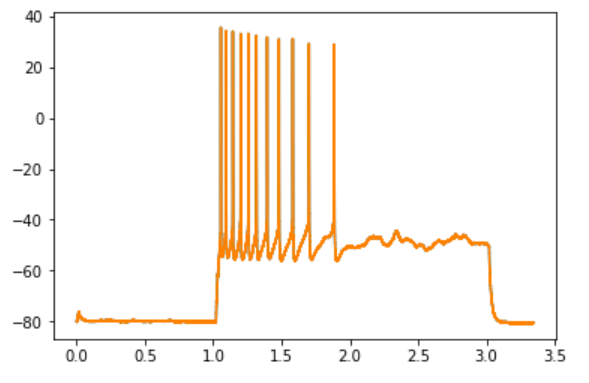
\includegraphics[]{chapters/app_tex/Allen_rush}
\begin{figure}
    \begin{center}
    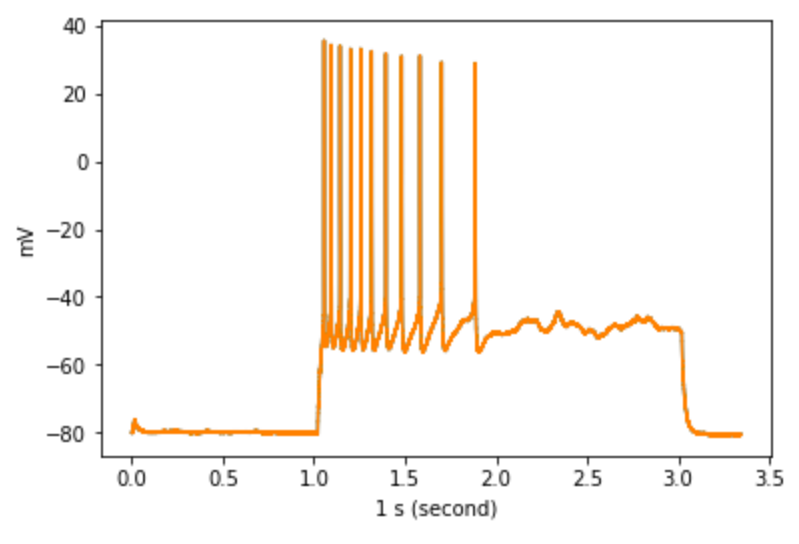
\includegraphics[width=0.6\linewidth]{figures/multi_spiking_large_allen}
    \caption{A voltage recording from a supra-threshold experiment waveform used as a basis for the Allen Brain Institute cell types data base. Publication Gouwens rat \cite{gouwens2018systematic}}
    \label{fig:adaptionm}
    \end{center}
\end{figure}    

\begin{figure}  
    \begin{center}
    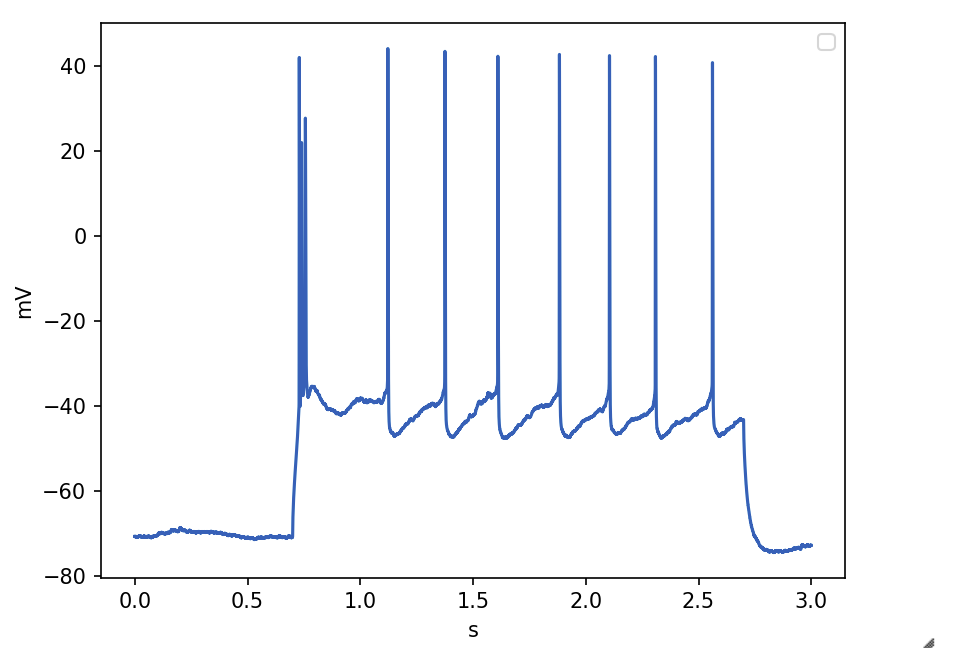
\includegraphics[width=0.6\linewidth]{figures/multi_spiking_large_bbp}
    \caption{Another example of a supra threshold experimental protocol. Publication Jouvanile rat \cite{toledo}}
    \label{fig:bbp_trace_adaption_late_spike}
    \end{center}
\end{figure}    

In order to identify electrical measurements or "features" that were responsible for the most variance in models and in-vitro, we performed Sparse Principle Component Analysis \cite{zou2006sparse} on the combined pool of model and in vitro experiments. 



\subsubsection{sources of disagreement}

The key advantage of using sparse PCA is the results are readily interpret able. A common sceanario in regular Principal Component Analysis is you may obtain a low dimensional embedding plot made from unit rotation vectors that maximize variance, but no way of relating the reduced dimensions back to the sources of variance in the system of interest. 

Sparse PCA yields an interpretable list of features, that build the principle components. This list of features is ranked and sorted with respect to their total contributions to the Eigen Vectors. Since two Eigen Vectors where made these are.

Principle component 1 had non zero loadings for ranked (highest to lowest).
The first Eigen Vector does not facilitate discrimination between models and experiments, but the second Eigen Vector spaces models and experiments into three seperate clusters.
\begin{verbatim}
upstroke_t_1.5x allen 
peak_t_1.5x allen 
threshold_t_1.5x allen 
fast_trough_t_1.5x allen 
fast_trough_t_3.0x allen 
upstroke_t_3.0x allen 
peak_t_3.0x allen 
threshold_t_3.0x allen 
peak_indices_1.5x efel 
min_AHP_indices_1.5x efel 
\end{verbatim}


Principle component 2 had non zero loadings for ranked (highest to lowest)
$
fast_trough_index_1.5x allen 
peak_index_1.5x allen 
upstroke_index_1.5x allen 
threshold_index_1.5x allen 
fast_trough_index_3.0x allen 
peak_index_3.0x allen 
upstroke_index_3.0x allen 
threshold_index_3.0x allen
$
These are the weighted features that were used to make Eigen vectors 1 and 2, are responsible for most of the variance. Interestingly these features are mostly belonging to the Allen SDK, with two exceptions: $peak_indices_1.5x$ $min_AHP_indices_1.5 \times$ belonging to EFEL efel 

Move to Discussion 
Another observation is that a small majority of features used to create the sparse Eigen Vectors, are in the range of $1.5$ * rheobase, and slightly fewer are features from a $3.0\times$ rheobase experiment. I believe this is because, larger spike time variability $C_{V}$ is expressed in intermediate ranges of current injection. Under the highest current injections, high frequency evenly spaced spikes are likely, although spike frequency adaption is possible, the higher current may force to spikes to occur promptly after their refractory period, and in this case you might observe diminishing amplitude of spikes with increasing stimulus duration.

At $1.5 \times rheobase $ I believe there to be more spike time variation, at $3.0 \times rheobase $  I believe there to be more spike amplitude variation.


%Scientific insight is well-served by the discovery and optimization of abstract models that can reproduce experimental findings. NeuroML (NeuroML.org), a model description language for neuroscience, facilitates reproducibility and exchange of such models by providing an implementation-agnostic model description in a modular format. NeuronUnit (neuronunit.scidash.org) evaluates model accuracy by subjecting models to experimental data-driven validation tests, a formalization of the scientific method. 


% After applying dimensionality reduction to this very high dimensional feature space, we show that the real (biological neurons) and simulated (model neurons) recordings are easiley and fully discriminated by eye or any reasonable classifier.  

% Are they still discernable?
972 models, 448 experiments.

\subsubsection{Sparse PCA}
Interestingly models and experiments clustered separately to each other in the low dimensional space. That is to say models and data were easily separable in the direction of the 2nd Eigen Vector.

%The first principle component 
Models and experiments shared the same breadth of variability across the first principal component, with only slightly more variance in the experiments than in the data. Allen cell types experiments seemed to encompass the most variability out of models and experiments across all data sets.


Models clustered tightly and varied less

Sparse PCA revealed five overlapping different groups of neuronal identity's, and three non overlapping clusters.

Although imputation was successfully used to avoid dropping a large number of samples, about half of all initial BBP/Allen models data types were excluded from a final analysis, because they did not all capable of meeting inclusion criteria.  

There was one group of Allen cell type experiments that clustered on their own, making one set of the cluster.

sparse PCA 2nd Eigen Vector. 
%Consequently, not a single model neuron produced physiological responses that could be confused with a biological neuron. Was this a defect of the model design (e.g. key mechanisms unaccounted for) or of model parameterization? We found that if we introduced models that were revised via optimization the revised models overlapped with the distribution of biological neurons, and were mostly classified as such. 
Disagreement between models and in-vivo neurons may reflect limitations of model design and can be investigated by probing the key features used by classifiers to distinguish these two populations. 

\begin{figure}    
\begin{center} 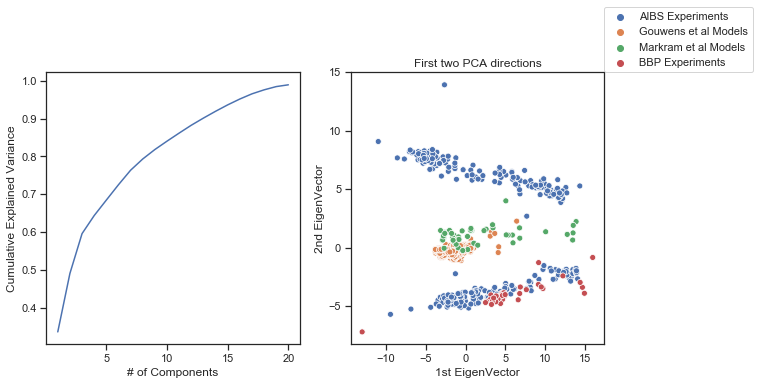
\includegraphics[width=1.0\linewidth]{figures/cortical_model_data_agreement_52_1}
    \caption{}
    \label{fig:}
\end{center}
\end{figure}    
\begin{figure}    
    \begin{center}
    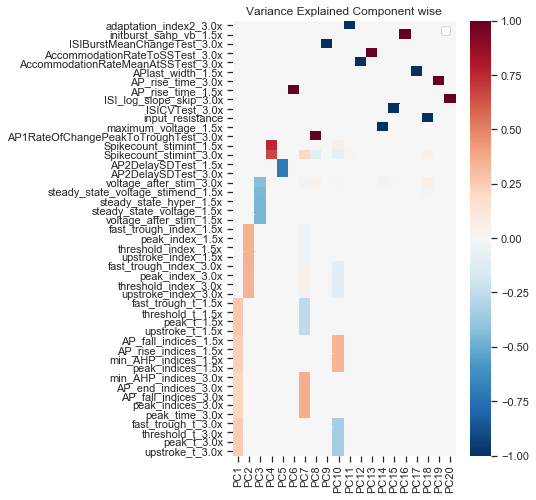
\includegraphics[width=1.0\linewidth]{figures/cortical_model_data_agreement_54_1.png}
    \caption{}
    \end{center}
\end{figure}    
\cite{wang2019sag}

\begin{figure}
    \centering
    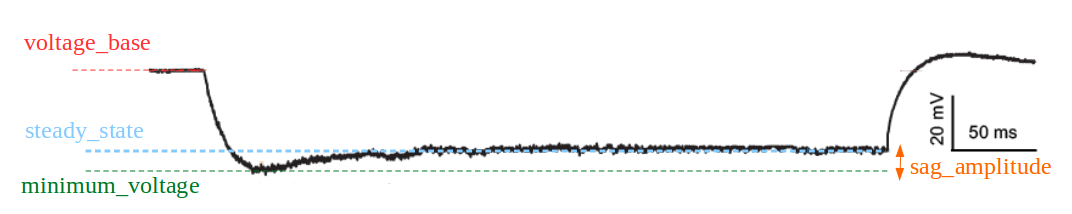
\includegraphics{figures/sag_amplitude}
    \caption{Caption}
    \label{fig:sag_amplitude}
\end{figure}

\begin{figure}
    \centering
    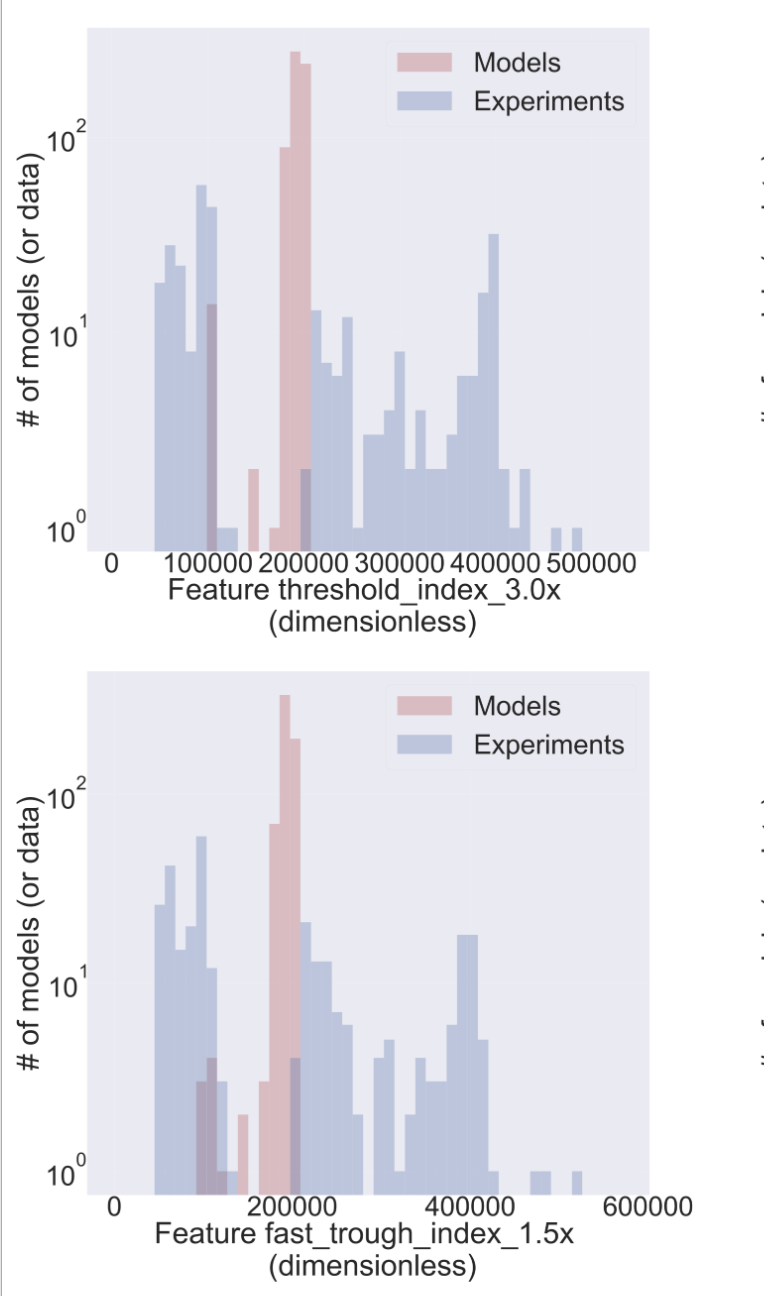
\includegraphics{figures/features_that_disagree}
    \caption{Caption}
    \label{fig:from_poster_disagree}
\end{figure}




\begin{itemize}
    \item upstroke\_t\_1.5x allen feature
    \item  peak\_t\_1.5x allen feature
    \item threshold\_t\_1.5x allen feature
    \item fast\_trough\_t\_1.5x allen feature
    \item fast\_trough\_t\_3.0x allen feature
    \item upstroke\_t\_3.0x allen feature
    \item peak\_t\_3.0x allen feature
    \item threshold\_t\_3.0x allen feature
    \item peak\_indices\_1.5x efel feature
    \item min\_AHP\_indices\_1.5x efel feature
\end{itemize}


\begin{itemize}

    \item fast\_trough\_index\_1.5x allen feature
    \item fast\_trough\_index\_3.0x allen feature
    \item threshold\_index\_1.5x allen feature
    \item peak\_index\_1.5x allen feature
    \item upstroke\_index\_1.5x allen feature
    \item peak\_index\_3.0x allen feature
    \item upstroke\_index\_3.0x allen feature
    \item threshold\_index\_3.0x allen feature
\end{itemize}



3.3
\include{chapters/NU_BPP_fusion_L5PC}
Section 4
4.1
\include{chapters/Discussion_significance_of_results}
Section 5
Optional conclusion
%-----------------------back matter
{\singlespace
% Making the references a "part" rather than a chapter gets it indented at
% level -1 according to the chart: top of page 4 of the document at
% ftp://tug.ctan.org/pub/tex-archive/macros/latex/contrib/tocloft/tocloft.pdf
\addcontentsline{toc}{part}{REFERENCES}
\bibliographystyle{chapters/minimal}
\bibliography{dis}}
\renewcommand{\chaptername}{APPENDIX}
\addtocontents{toc}{APPENDIX \par}
%\appendix
%\include{chapters/appendix1}
\include{vita}
\end{document}
